%%%%%%%%%%%%%%%%%%%%%%%%%%%%%%%%%%%%%%%%%
% This document provides a sample senior 
% thesis proposal template for use
% by Allegheny's Computer Science majors.
%
% This template was adopted from Jeremie Gillet
% Ref: https://github.com/oist/LaTeX-templates
%
% Author: Janyl Jumadinova
% Last Updated: 15 October 2021
%
%%%%%%%%%%%%%%%%%%%%%%%%%%%%%%%%%%%%%%%%%

%----------------------------------------------------------------------------------------
%	PACKAGES AND OTHER DOCUMENT CONFIGURATIONS
%----------------------------------------------------------------------------------------

\documentclass[12pt,oneside]{book} % 12 pt font, one-sided book style
\usepackage[a4paper, includehead, headheight=0.6cm, inner=3cm ,outer=2.5cm, top=2.5 cm, bottom=2.5cm]{geometry}  % Changing size of document
\usepackage[english]{babel} % The document is in English
\usepackage[utf8]{inputenc} % UTF8 encoding
\usepackage[T1]{fontenc} % Font encoding

\usepackage{graphicx} % For including images
\graphicspath{{./images/}} % Specifies the directory where images are stored

\usepackage{longtable} % tables that can span several pages
\usepackage[bf]{caption} % caption: FIG in bold
\usepackage{fancyhdr} % For the headers

\newcommand{\numberedchapter}{ % Preparation for numbered chapters
	\cleardoublepage % To make sure the previous headers are passed
	\fancyhead[RE]{{\bfseries \leftmark}}% Headers for left pages
	\fancyhead[LO]{{\bfseries \rightmark}}}% Headers for right pages
\newcommand{\unnumberedchapter}[1]{ % Preparation for unnumbered chapters
	\cleardoublepage % To make sure the previous headers are passed
	\addcontentsline{toc}{chapter}{#1} % Also adds the chapter name to the Contents
	\fancyhead[RE]{{\bfseries #1}} % Headers for left pages
	\fancyhead[LO]{}}%Headers for right pages

\def\code#1{\texttt{#1}}

\usepackage{emptypage} % No headers on an empty page

\usepackage{eso-pic} % For the background picture on the title page
\newcommand\BackgroundPic{%
\put(0,-120){%
\parbox[b][\paperheight]{\paperwidth}{%
\vfill
\centering

\includegraphics[width=4in]{images/logo}%
\vfill
}}}

\usepackage{hyperref} % Adds clickable links at references

%----------------------------------------------------------------------------------------
%	ADD YOUR CUSTOM VALUES, COMMANDS AND PACKAGES
%----------------------------------------------------------------------------------------

% Open preamble/mydefinitions.tex and enter some values (name, thesis title...) 
% and include your own custom LaTeX functions and packages

%----------------------------------------------------------------------------------------
% values for the proposal
%----------------------------------------------------------------------------------------

\newcommand{\name}{Noor Buchi} % Author name
\newcommand{\thesistitle}{AFLuent: An Implementation and Evaluation of Automated Fault Localization Tool in Python} % Title of the thesis
\newcommand{\submissiondate}{\today} % Submission date "Month, date year"
\newcommand{\supervisor}{Dr. Gregory Kapfhammer} % First reader's name
\newcommand{\cosupervisor}{Maria Kim Heinert} % Second reader's name


%----------------------------------------------------------------------------------------
%	BIBLIOGRAPHY STYLE 
%----------------------------------------------------------------------------------------


\bibliographystyle{acm}

%----------------------------------------------------------------------------------------
%	YOUR PACKAGES (be careful of package interaction)
%----------------------------------------------------------------------------------------

\usepackage{amsthm,amsmath,amssymb,amsfonts,bbm}% Math symbols

%----------------------------------------------------------------------------------------
%	YOUR DEFINITIONS AND COMMANDS
%----------------------------------------------------------------------------------------

% New Commands
\newcommand{\bea}{\begin{eqnarray}} % Shortcut for equation arrays
\newcommand{\eea}{\end{eqnarray}}
\newcommand{\e}[1]{\times 10^{#1}}  % Powers of 10 notation


\begin{document}

%----------------------------------------------------------------------------------------
%	TITLE PAGE
%----------------------------------------------------------------------------------------

\pagestyle{empty} % No page numbers
\frontmatter % Use roman page numbering style (i, ii, iii, iv...) for the preamble pages

\begin{titlepage}
\AddToShipoutPicture*{\BackgroundPic}
\begin{center}
\vfill
{\large \scshape Allegheny College \\ Department of Computer Science }\\[1.4cm]
{\Large Senior Thesis}\\[0.5cm]
\rule{\textwidth}{1.5pt}\\[0cm]
{\huge \bfseries \thesistitle \par \ }\\[-0.5cm]
\rule{\textwidth}{1.5pt}\\[2.5cm]
\hfill  by\\[1cm]
\hfill  {\large \bfseries\name}\\
\vfill
{\hfill \large Project Supervisor: \textbf{\supervisor}} \\ 
\ifx\cosupervisor\undefined\else{\hfill \large Co-Supervisor: \textbf{\cosupervisor}} \\ \fi
\vspace{1cm}
\hfill  \submissiondate
\end{center}
\end{titlepage}


\pagestyle{fancy} % Changes the headers
\fancyhf{}% Clears header and footer
\fancyhead[RO,LE]{\thepage} % page number on the outside of headers

%-------------------------------------------------------------------------------
%	PREAMBLE PAGES (delete unnecessary pages)
%   preamble pages besides abstract are optional
%-------------------------------------------------------------------------------

\unnumberedchapter{Abstract} 
\chapter*{Abstract} 

Provide a concise summary of your  research project of approximately 250 words. 
Remember that the abstract is {\it not\/} an introduction, it is a {\it summary\/} of the entire document, including the results and future direction of the project.
\unnumberedchapter{Acknowledgment}
\chapter*{Acknowledgment}

Many thanks to Dr. Kapfhammer for his invaluable assistance in the development of this
idea, the implementation, and evaluation of this tool. His continuous advice
and encouragement throughout the research was crucial in pointing me in the
right direction. I'm grateful for the time and effort he dedicated to ensure the
completion of this project. I'm also thankful for the Allegheny College
Computer Science faculty and my classmates for all their support and willingness
to give constructive feedback.

\unnumberedchapter{Abbreviations} 
\chapter*{Abbreviations} 
% TODO: add more if needed
\begin{longtable}{rl}
AFL & automated fault Localization\\
SBFL & spectrum-based fault localization
\end{longtable}
\unnumberedchapter{Glossary} 
\chapter*{Glossary} 

% Break up this table into several ones if it takes up more than one page
\begin{center}
\begin{longtable}{r p{0.58 \textwidth}}
Dipole Blockade & Phenomenon in which the simultaneous excitation of two atoms is inhibited by their dipolar interaction. \\
Cavity Induced Transparency & Phenomenon in which a cavity containing two atoms excited with light at a frequency halfway between the atomic frequencies contains the number of photons an empty cavity would contain.  \\ 
\end{longtable}
\end{center}

\cleardoublepage
\thispagestyle{empty} % Page style needs to be empty for this page

\vspace*{8cm}
\hfill
\begin{parbox}{0.6\textwidth}{
\begin{flushright}


\end{flushright}}
\end{parbox}




%-------------------------------------------------------------------------------
%	LIST OF CONTENTS/FIGURES/TABLES
%-------------------------------------------------------------------------------

\unnumberedchapter{Contents}
\tableofcontents % Write out the Table of Contents
\unnumberedchapter{List of Figures}
\listoffigures % Write out the List of Figures
\unnumberedchapter{List of Tables}
\listoftables % Write out the List of Tables

%-------------------------------------------------------------------------------
%	THESIS MAIN TEXT
%-------------------------------------------------------------------------------

\addtocontents{toc}{\vspace{2em}} % Add a gap in the Contents, for aesthetics
\mainmatter % Begin numeric (1,2,3...) page numbering

%----------------------------------------------------------------------------------------
%	START DELETE TEXT
%----------------------------------------------------------------------------------------

\section*{Template Overview}

You should first modify the documents in the preamble, things that appear before the main text as detailed below. 

\textbf{Front page}: use the one provided in this template, after changing the values like names in the file \texttt{preamble/mydefinitions.tex}.

\textbf{Abstract}: There should be a single paragraph of about 250 words, which concisely summarizes the entire proposal, written in the file \texttt{preamble/abstract.tex}.

\textbf{Acknowledgments, Abbreviations, Glossary, Dedication} preamble pages are optional and can be used at the author's discretion. 

The main text of the proposal should be stored in the ``SeniorThesis.tex'' document. The following descriptions are sections that must be included in the thesis document.

\textbf{Bibliography}: The bibliography should include all references cited in the text (as \cite{dasgupta2015comrade}) and it should not include references that have not been cited. ACM referencing style should be used when preparing the bibliography. We recommend using BibTeX or BibLaTeX and using the file \texttt{preamble/bibliography.bib}.

%----------------------------------------------------------------------------------------
% STOP DELETE
%----------------------------------------------------------------------------------------

%\numberedchapter{Introduction} % Title of the numbered chapter
\chapter{Introduction}
\label{ch:intro}

\section{Motivation}
\label{sec:motivation}

Debugging is a task that every developer and software engineer will have to go
through while writing code. It's often a
tedious process that involves manually checking the code and running it multiple
times to simply find the location of the error in the code. More formally,
debugging ``involves analyzing and possibly extending the given program that
does not meet the specification in order to find a new program that is close to
the original and does satisfy the specifications... it is the process of
`diagnosing the precise nature of a known error and then correcting it' '' \cite{Hailpern2002Debugging}.
Finding possible solutions to fix the fault would then be the next step
in the debugging process. In Postman's 2020 State of the API Report,
developers reported allocating seventeen percent of their time
debugging and manually testing their code.
Fig \ref{fig:development_time} demonstrates that debugging makes up the
second most time-consuming task for API developers.
In an effort to facilitate and automate this process, different tools have been
created to guide the developer in locating error(s) and suggesting how to go
about fixing them. Solving this problem can significantly increase the
efficiency of experienced developers and increase the quality of the code they
ship. Additionally, a solution can help in decreasing the time spent on
debugging and allow developers to focus on other important tasks.
Beginner and novice developers can also benefit greatly from tools
that facilitate the debugging process, which could ease the learning process and help
them avoid making mistakes. Overall, contributions to this field of study could
assist developers and software engineers of all levels.
With special concentration on novice and beginner developers in an educational
environment, this research implements and evaluates a tool focused on helping
developers find bugs in their code.

% TODO: check all citations
% TODO: create citation
\begin{figure}[!htb]
	\begin{center}
		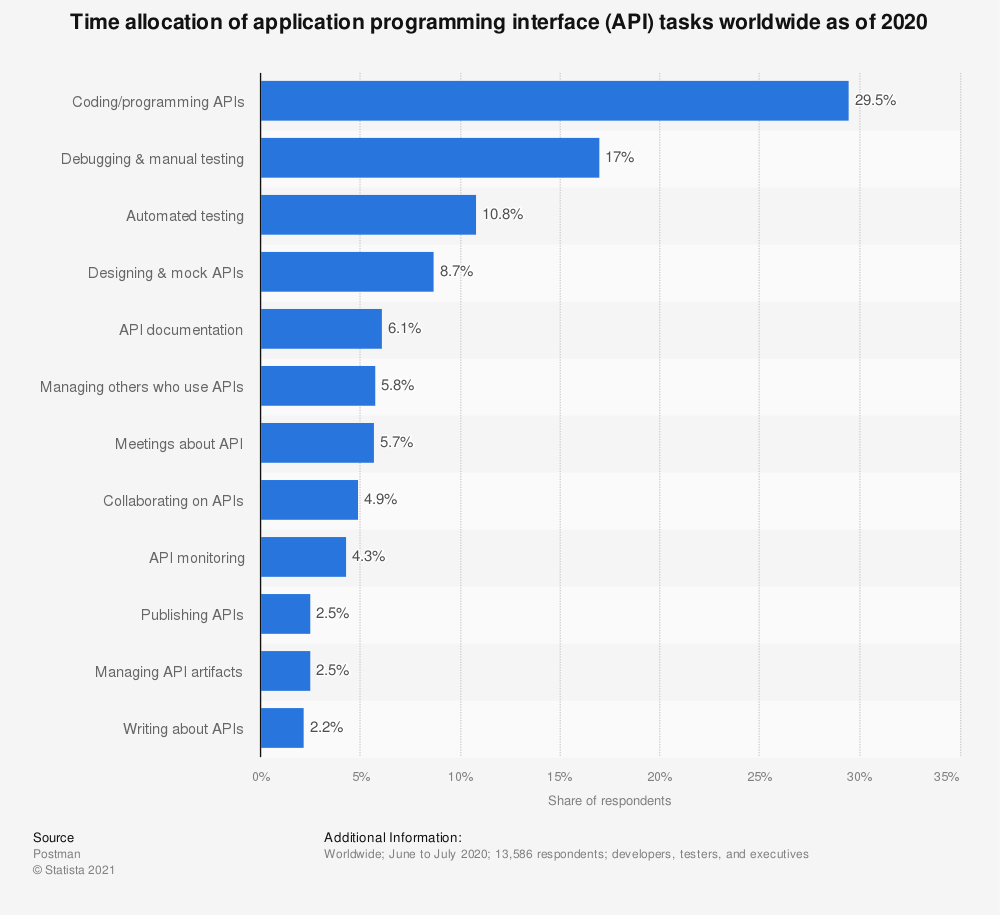
\includegraphics[width=\textwidth]{dev_time_stat.png}
		\caption{\label{fig:development_time} API Developers Time Allocation}
	\end{center}
\end{figure}

\section{Background}
\label{sec:background}

\subsection{Debugging and Fault Localization}
\label{subsec:DebuggingAndAFL}

The debugging process for developers typically starts when a ``bug'',
unexpected/incorrect behavior has been observed. One of many ways to check
whether incorrect behavior is taking place is through unit testing. This type of
testing consists of a set of test cases that check the different functionalities of the
code by asserting that expected output and actual output match. When a test case
fails due to a mismatch in the assertion, the search for the causing bug begins.
This research focuses on this crucial step in debugging and aims to guide the
search process by setting priority locations for the developers to search in.

Debugger tools have often been used to find and fix bugs in code, and while they
have several benefits, they also have drawbacks. Debuggers provide the developer
with a way to essentially pause the runtime of a program using breakpoints to display
information about the state of different variables and function call stack.
Through debuggers, developers can run the code line by line until an unexpected
behavior is detected. There is no denial that debuggers are very effective,
however, using them can be time-consuming, especially for complex bugs.
Additionally, debuggers require that the code is run during the debugging
process which could increase the time needed to debug and might not always be
feasible. With these drawbacks in mind, several automated fault localization (AFL)
algorithms and approaches have been studied to increase the
efficiency of the debugging process.

% TODO: find the sources that explores different types of AFL
Automated Fault Localization approaches perform different types of analysis to
the code and attempt to find the location of existing faults. Some approaches
use trained artificial intelligence models to assess the code and make
predictions on where some faults may exist. Others construct and analyze
abstract syntax trees to look for potential errors. On the other hand,
approaches such as spectrum-based fault localization rely on data collected
during the runtime of the code to ``identify the part of the program whose
activity correlates most with the detection of errors'' \cite{ABREU20091780}.
More specifically, the results of the program's test suite are used to find this
correlation. This latter approach is the focus of this research, where a
spectrum-based automated fault localization tool is implemented.

\subsection{Spectrum Based Fault Localization}
\label{subsec:SpectrumBased}

The reliance of spectrum based fault localization (SBFL) on data already
collected during running and testing reduces the overall cost of debugging since
there is no need to rerun the code. When focusing on collected test suite data,
SBFL becomes even more applicable since it can be integrated with many unit test
frameworks. In addition to the per-test outcome of a test suite, per-test
coverage data is also used in SBFL to identify which lines are executed by each
test case. Once this data is collected following a test suite run, SBFL assesses
the suspiciousness of code blocks depending on how many failing test cases run
those blocks. From a logical point of view, the block/line of code executed the
most by a failing test case is the most likely to contain the fault. SBFL also
uses various equations to calculate and quantify the
suspiciousness of blocks of code. The equations are expressed as functions of
elements, where each element is the line or block of code under inspection. The
functions typically include the following variables\cite{Wong2014DStar}:

\begin{center}
	\textbf{N$_{CF}$}: number of failed test cases that execute/cover the element

	\textbf{N$_{UF}$}: number of failed test cases that do not execute/cover the element

	\textbf{N$_{CS}$}: number of passed test cases that execute/cover the element

	\textbf{N$_{US}$}: number of passed test cases that do not execute/cover the element
\end{center}

% TODO: needs updated when the fourth equation is picked
Using these variables, past research has come up with many equations to
calculate elements' suspiciousness scores. This research focuses on three main
popular equations and adds support for them in AFLuent. The reasoning behind the
equation choices is further discussed in Related Works, however, this section
will give an overview of how each looks like.

\subsubsection{Tarantula}
\label{subsubsec:Tarantula}
\begin{figure}[!htb]
	\begin{center}
		\begin{equation}
			Tarantula(element) = \frac{\frac{\textbf{N$_{CF}$}}{\textbf{N$_{CF}$} + \textbf{N$_{UF}$}}}{\frac{\textbf{N$_{CS}$}}{\textbf{N$_{CS}$}+\textbf{N$_{US}$}} + \frac{\textbf{N$_{CF}$}}{\textbf{N$_{CF}$}+\textbf{N$_{UF}$}}}
		\end{equation}
		\caption{\label{fig:tarantulaEquation} Tarantula Equation\cite{Jones2005TarantulaEval}}
	\end{center}
\end{figure}

The Tarantula equation is one of the most popular Coverage based fault localization
formulas to calculate suspiciousness scores of code elements. It uses the
variables listed previously to generate a score between 0 and 1, where 0 is
assigned for non-suspicious elements and 1 is assigned for most suspicious ones.

\subsubsection{Ochiai}
\label{subsubsec:Ochiai}
\begin{figure}[!htb]
	\begin{center}
		\begin{equation}
			Ochiai(element) = \frac{\textbf{N$_{CF}$}}{\sqrt{(\textbf{N$_{CF}$}  + \textbf{N$_{UF}$}) \cdot (\textbf{N$_{CF}$}  + \textbf{N$_{CS}$})}}
		\end{equation}
		\caption{\label{fig:ochiaiEquation} Ochiai Equation\cite{Abreu2006Ochiai}}
	\end{center}
\end{figure}

Ochiai is another equation used to calculate suspiciousness scores between 0 and
1. It relies on similar code test and coverage variables as the Tarantula
equation. AFLuent supports using this equation in its automated fault
localization process. More discussion around Ochiai can be found in the related
works section.

\subsubsection{DStar}
\label{subsubsec:DStar}
\begin{figure}[!htb]
	\begin{center}
		\begin{equation}
			Dstar(element) = \frac{(\textbf{N$_{CF}$})^{\ast}}{\textbf{N$_{CS}$} + \textbf{N$_{UF}$}}
		\end{equation}
		\caption{\label{fig:dstarEquation} DStar Equation\cite{Wong2014DStar}}
	\end{center}
\end{figure}

The DStar equation also results in a score between 0 and 1, however, it includes
a new variable represented as the * symbol. This variable can give more
weight to \textbf{N$_{CF}$} and can be set to any number. However, the
researchers suggested that * is set to 2 or 3.

\subsection{SBFL in Action}
\label{subsec:SBFLinAction}

\begin{figure}[!htb]
	\begin{center}
		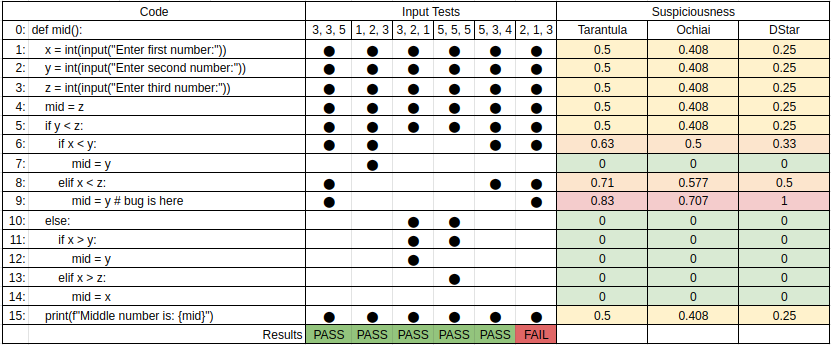
\includegraphics[width=\textwidth]{SFL_example.png}
		\caption{\label{fig:sbfl} Applied Example of SBFL Equations}
	\end{center}
\end{figure}

With the discussed equations and techniques to calculate suspiciousness in mind,
the following example will demonstrate and discuss how AFLuent will utilize unit
test and coverage data to locate faults in a program. Fig\ref{fig:sbfl_example}
shows a sample python program to find the middle value
from three integers. The program contains a bug on line 9 where the wrong middle
number is detected. The figure also shows six different test cases that pass
various inputs to the function and check whether the actual output matches the
expected. The results of each test is found on the last row of the table.
Additionally, the large dots under the Input Tests column illustrate the concept
of code coverage. For each line of code and test input, a dot in the cell means
that the line was executed when this input was passed. On the rightmost column
of the table, suspiciousness scores for each line are calculated using the three
formulas (Tarantula, Ochiai, and DStar). High suspiciousness scores are also
highlighted in warmer colors. Overall, all three equations are able to detect
that line 9 is the most suspicious and is likely the cause of the test failure.

\subsection{SBFL Criticism}
\label{subsec:Criticism}

While SBFL can provide great insight for developers looking to debug their code,
it's not always reliable or applicable. In the case where a test suite hasn't
been fully implemented, the output of SBFL may not narrow down potentially faulty
code to a single line. Additionally, ties in suspiciousness scores between lines
and blocks may come up, which may not offer the developer any valuable output.
Overall limitations of SBFL will be discussed in Related Works and acknowledged
while evaluating the outcome of this research.

\section{Main Aims}
\label{sec:aims}

% TODO: maybe talk about the other existing python tool?
With the demonstrated importance of debugging tools and strategies that increase
developer efficiency, this research implements and evaluates an AFL tool to
assist in debugging code. AFLuent is built using  Python programming
language and uses SBFL approach to identify faults in a
% TODO: create citation
program. Stack Overflow 2021 Developer Survey identified Python as the third
most used programming/markup language used by developers worldwide. With that in
mind, an automated fault localization tool in Python can reach a wide audience
in various fields such as data science and AI who may have various levels of
experience. By implementing AFLuent using Python, powerful libraries and
packages such as Pytest and Coverage.py can be used to collect test suite data
in order to calculate suspiciousness.

Following the implementation of AFLuent, this research evaluates the
tool's performance and accuracy. Several open source projects
available on GitHub are handpicked to run AFLuent against. A representative
sample of projects with various sizes and relevance will be used to collect
data. Mutation testing libraries are used to introduce bugs into the code,
following that step, AFLuent uses the resulting test suite data to identify the
introduced fault. Through this process, AFLuent's performance and ability to
correctly identify and rank suspicious statements/and blocks is assessed.

\section{Research Questions}
\label{sec:researchq}

Throughout the implementation, testing, and evaluation of AFLuent, this research
presents the following research questions and aims to answer each in detail.
There are two main research questions that focus on different aspects of
AFLuent. Each one is further split into sub-questions to facilitate organization.

\begin{center}
	\emph{RQ1. What are the most accurate available techniques to automate the process of
	fault localization using test coverage data?
	}
\end{center}

This general research question focuses on the core implementation and
evaluation of AFLuent. Considering that many SBFL strategies and formulas can be
used, finding the most suitable and most accurate one in detecting bugs is one
of the goals of this research. In order to answer this question,
available literature on SBFL is analysed and the most popular and cited formulas
are included in the implementation of AFLuent. Answering this question also
requires that each approach is evaluated through an experiment section.
Since this research question is includes two separate sections, it's further split into
smaller sub-questions discussed below.

\begin{center}
	\emph{RQ1.1. What are the four most popular formulas for code suspiciousness
	created and evaluated by past literature?
	}
\end{center}

Available literature surrounding SBFL is reviewed to identify four
different formulas used to calculate suspiciousness scores using test coverage
information. Each of these formulas are integrated into AFLuent where the user
is able to select the approach to use while debugging. The popularity, accuracy,
and performance as found in past work are the main criteria used to pick the top
formulas.


\begin{center}
	\emph{RQ1.2.  What is the accuracy and efficiency of the chosen
	formulas when applied to Python projects?
	}
\end{center}

To ensure correctness and effectiveness, the implemented formulas in AFLuent are
evaluated through experiments that measure their accuracy in sorting suspicious
statements and blocks. More specifically, the formulas will be assessed in in
the context of Python projects that use the Pytest unit testing framework.
More details on this research question can be found in the evaluation section.

While RQ1 involves technical details around implementation and assessment of
AFLuent, RQ2 focuses on user experience. Since the target audience of AFLuent is
beginner developers, it's important to ensure that AFLuent produces meaningful
and clear results that guide developers. In order to answer this question,
AFLuent adopts various standards in interacting with the user through console
output, as well as error messages and warnings.

\begin{center}
	\emph{RQ2. How can automated fault localization techniques be implemented in
	Python as a novice developer friendly tool?
	}
\end{center}

In addition to ensuring a smooth user experience while utilizing AFLuent
functionalities, setup process and usage of the tool AFLuent is simplified to
facilitate installation. Clear and descriptive documentation is also a crucial
step in making AFLuent accessible available for new users.

\section{Thesis Outline}
\label{sec:outline}

Starting with a literature review, this research identifies important sources
that guide the implementation of AFLuent and discusses their use. Additionally,
the methods section extensively describes how AFLuent is implemented and the
steps taken to ensure it functions correctly while being up to industry
standards. The different tools used to build and test AFLuent are also
discussed in the methods sections. Following that, the evaluation section
describes the steps taken to evaluate AFLuent by testing the tool and
collecting data regarding it's output. The evaluation section also includes an
analysis of the results of the evaluation and various plots and charts that
show the findings.
 % Introduction (first numbered chapter)

%\numberedchapter{Related Work}
\chapter{Related Work}
\label{ch:relatedwork}

Automated fault localization in general and more specifically spectrum based
fault localization have extensive literature exploring the different approaches
to facilitate debugging and increase developer efficiency. Considering that
AFLuent relies on many concepts developed by this literature, this section will
explore and discuss how past work shapes AFLuent. Several sections are created
to for specific area of literature.

\section{Automated Fault Localization}
\label{sec:AFLlit}

Survey papers are one of the many ways that assist in better
understanding and having a wide collection of the existing
literature surrounding automated fault localization (AFL).
Wong et al. \cite{wong2016survey} explores the variety of AFL approaches and
surveys research completed in that area between 1977 and 2014. The survey paper finds and
discusses more than 334 different papers in many approaches in AFL.
\begin{figure}[!htb]
	\begin{center}
		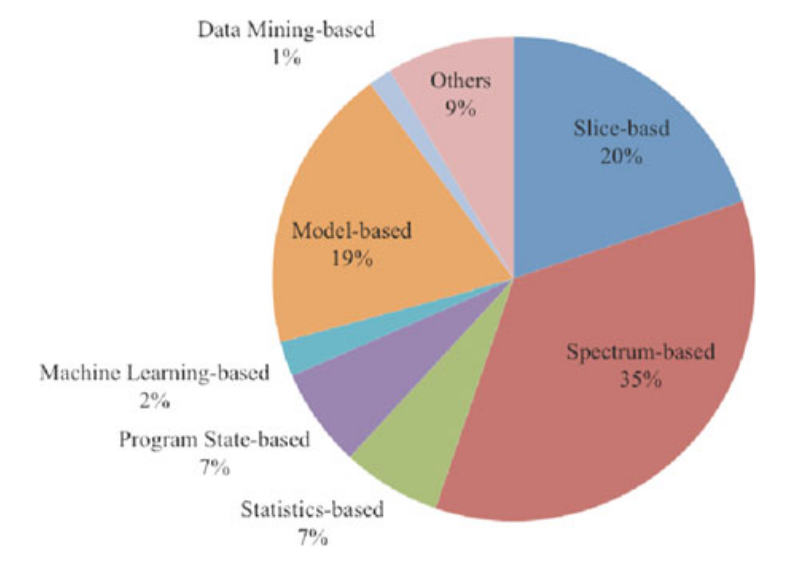
\includegraphics[width=10cm]{wong_pie_chart.png}
		\caption{\label{fig:wong_breakdown} AFL papers found by Wong et al. \cite{wong2016survey}}
	\end{center}
\end{figure}

A breakdown of the found research is shown in Fig. \ref{fig:wong_breakdown}, where the
majority of found papers are focused on Spectrum-Based Fault Localization (SBFL).
Overall this research provides a great
starting point to find and compare the different types and approaches of AFL.
Another benefit of this resources is that
Wong et al. \cite{wong2016survey} expands on the types of SBFL
and reviews key literature that contributes show the benefits and drawbacks of
each approach.

\subsection{SBFL Approaches}
\label{subsec:sbfl}

\subsubsection{Similarity Coefficient Based Technique}
\label{subsubsec:coefficient_based}

One of the most relevant SBFL techniques described by Wong et al.
\cite{wong2016survey} is similarity coefficient based ones. Generally, these approaches
seek to quantify how close ``the execution pattern of a statement is to the
failure pattern of all test cases'', where the the closer they are the more
likely that this statement to contain the error. In order to create a
measurement of closeness, several equations have been developed and evaluated by
past literature. Fig. \ref{fig:sbfl_eq} shows some of the equations reviewed by
Wong et al in, however, more popular formulas have been developed that
required the developer to analyze less code before finding the fault. Despite
the existence of many Similarity Coefficient formulas, Yoo et al.
\cite{yoo2014no} concludes in an extensive evaluation study that there is no
formula that outperforms all others in all circumstances. With that in mind,
AFLuent gives the user the option to choose which approach to use and includes
a performance evaluation of each.

\begin{figure}[!htb]
	\begin{center}
		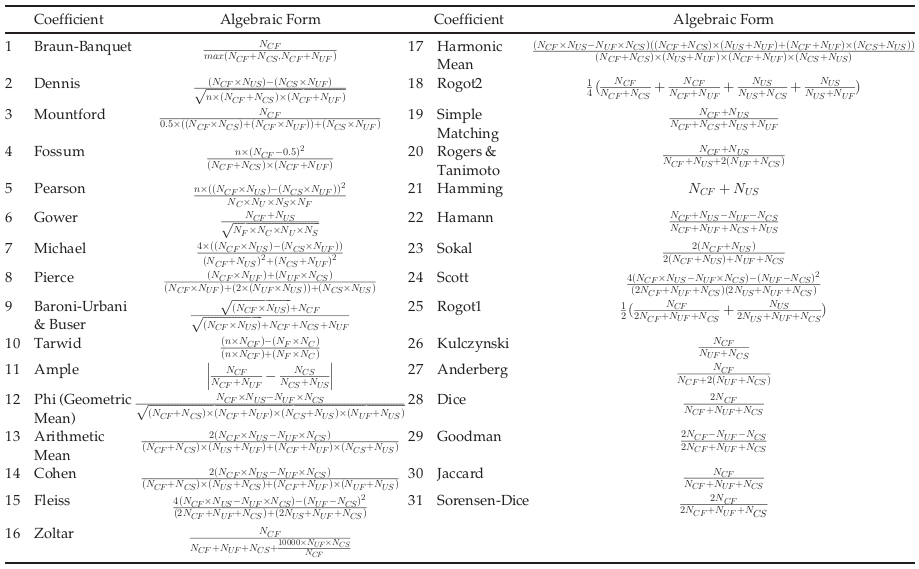
\includegraphics[width=\textwidth]{sfl_table.png}
		\caption{\label{fig:sbfl_eq} Coefficient Based Formulas \cite{wong2016survey}}
	\end{center}
\end{figure}

\subsubsection{Tarantula}
\label{subsubsec:tarantula_lit}

Starting off with the Tarantula formula (fig. \ref{fig:tarantulaEquation}), it's
one of the foundational equations that was introduced to attempt to visualize
suspicious statements using color ranges \cite{jones2002viz,
Jones2005TarantulaEval}. A tool using this equation was also implemented in Java
in order to scan code and assign colors to statements based on their
suspiciousness. The equation for Tarantula is made of two main ratios, the first
one being the number of failed tests that cover the element divided by the total
number of failed tests (\(\frac{\textbf{N$_{CF}$}}{\textbf{N$_{CF}$ +
\textbf{N$_{UF}$}}}\)). The other ratio used is number of passing tests that
cover the element divided by total number of passing tests
(\(\frac{\textbf{N$_{CS}$}}{\textbf{N$_{CS}$}+\textbf{N$_{US}$}}\)).
The equation is then assembled as seen in fig. \ref{fig:tarantulaEquation}.
To better understand how the equation works, we can look at the important terms
that have the largest influence in changing the output.The number of failed
tests that cover the element is clearly the main influencer here because it's
what causes the numerator to grow larger. This means that an increase in failed
tests that cover the element cause an increase in suspiciousness. Additionally,
a decrease in the number of failing tests that do not cover the element also
increase suspiciousness. Considering these two points, Tarantula gives a better
indicator of suspiciousness when there are fewer failures in tests covering
elements not under inspection. In addition to the logical analysis of the
equation previous works provide an empirical evaluation of Tarantula in
comparison to other formulas. Jones et al. \cite{Jones2005TarantulaEval}
compares the effectiveness and efficiency of Tarantula to techniques such as Set Union, Set
Intersection, and Nearest Neighbor. The results demonstrate that Tarantula
outperform the other Techniques where it provided a better guidance to the
developer. Using Tarantula a developer would need to manually
inspect fewer elements of the program compared to when using other approaches.

Another variation of Tarantula is also introduced in \cite{debroy2010grouping},
where grouping of suspicious elements is used to provide a better guide for
developers. In this modification, ``statements that are executed by the same
number of failed test cases are grouped together'', then suspiciousness scores
are used to sort elements within each group. By doing so, two layers of sorting
exist, the first one based on the number of failed tests covering the element,
and then the suspiciousness scores. The empirical results in Debroy et al.
\cite{debroy2010grouping} show a statistically significant improvement provided
by this grouping technique where the developer need to review less elements and
more faults are accurately detected. While Debroy et al. only applied the
grouping technique to Tarantula and a neural network-based approach, it could be
extended to include other similarity coefficient based techniques.

Overall, while other formulas outperform Tarantula as will be discussed,
incorporating this equation in AFLuent offers a starting point and a point of
comparison to other equations. One of the goals of AFLuent is to give the user
the ability to choose their most fitting approach to localize faults, and it's
useful to include Tarantula as one of the available options.

\subsubsection{Ochiai}
\label{subsubsec:ochiai_lit}

Ochiai is another similarity coefficient formula for SBFL that uses code
coverage information and test output to produce as suspiciousness score.
Originally used in computing genetic similarity in molecular biology and
evaluated in Abreu et al. \cite{Abreu2006Ochiai}, the equation for this approach
is shown in fog.\ref{fig:ochiaiEquation}. Similar to Tarantula, the number of
failing test cases that execute an element are the main factor in increasing
suspiciousness. The formula uses similar terms as Tarantula such as total number
of tests that cover the element, unlike Tarantula, however, it does not consider
successful tests that do not cover the element.
Papers such as \cite{Abreu2006Ochiai,ABREU20091780} also evaluate the
performance of Ochiai in comparison to other such as Tarantula, AMPLE, and
Jaccard. Another evaluation of Ochiai is done by Le et al. \cite{le2013theory}
where it was found to have a statistically significant improvement when compared
to Tarantula. The paper demonstrates that on average developers only need to
inspect 21.02\% of the source code before finding the fault.
AFLuent includes and implementation and evaluation of Ochiai to
validate that it performs as expected compared to the Tarantula technique.
Additionally, considering that Ochiai is considered a fairly accurate and
effective formula to detect faults, AFLuent takes advantage of the performance
it offers.

\begin{figure}[!htb]
	\begin{center}
		\begin{equation}
			Ochiai2(element) = \frac{\textbf{N$_{CF}$}\cdot{\textbf{N$_{US}$}}}{\sqrt{(\textbf{N$_{CF}$}  + \textbf{N$_{CS}$}) \cdot (\textbf{N$_{US}$}  + \textbf{N$_{UF}$}) \cdot (\textbf{N$_{CF}$}  + \textbf{N$_{UF}$}) \cdot (\textbf{N$_{CP}$}  + \textbf{N$_{US}$})}}
		\end{equation}
		\caption{\label{fig:ochiai2Equation} Ochiai2 Equation\cite{wong2016survey}}
	\end{center}
\end{figure}

In addition to the Ochiai formula in fig.\ref{fig:ochiaiEquation}, another
variation of Ochiai is identified and evaluated by \cite{naish2011model}. The
formula for Ochiai2 is shown in \ref{fig:ochiai2Equation} and it takes into
consideration all the possible outcomes of unit test coverage. Overall, this
variation is included in AFLuent to compare the performance between Ochiai2 and
the original formula and see if it provides an improvement in effectiveness.
Both Ochiai and Ochiai2 are relevant similarity coefficient-based approaches
that add variety to AFLuent and allow a representative evaluation of the tool
that takes in many different approaches..

\subsubsection{DStar}
\label{subsubsec:dstar_lit}

DStar (also written as D*) is another SPFL technique that utilizes code coverage
information of a program to locate and rank faults. The equation for this
approach can be found in fig.\ref{fig:dstarEquation}. Wong et al.
\cite{Wong2014DStar} introduce and extensively evaluate this approach in a 2014
paper that demonstrate it's effectiveness compared to other formulas. In the
process of constructing D*, the paper lists the factors involved in determining
suspiciousness of an element. The principles are as follows:
\begin{enumerate}
	\item Suspiciousness is directly proportional to the number of failed tests
	covering the element.
	\item Suspiciousness is inversely proportional to the number of successful tests
	covering the element.
	\item Suspiciousness is inversely proportional to the number of failed tests
	that do not cover the element.
	\item The number of failed tests covering the element should have the most
	weight in determining suspiciousness.
\end{enumerate}

Considering that multiplying \(\textbf{N$_{CF}$}\) by a constant to increase its
weight will not affect the ranking of statements, he authors argue that
rasing \(\textbf{N$_{CF}$}\) to a value * greater than
or equal to 1 would be more appropriate in increasing the weight of this
variable. The study continues by illustrating how increasing the value of *
produces more clear rankings that facilitate the debugging process by requiring
the developer to examine less elements in bot the best and worst case. However,
the authors also point out that this benefit of increasing teh value of * levels
off at a certain point depending on the size of the program under analysis.
The paper concludes by reviewing performance results showing that D* is more
effective than the previously discussed formulas (Tarantula, Ochiai, and
Ochiai2). With that in mind, D* offers the latest and most effective formula to
calculate suspiciousness compared to all others included in this research.
AFLuent implements D* to validate this step up in effectiveness in the context of
Python projects and gives the user the ability to use t.

\subsection{Combining Approaches}
\label{subsec:combining_approaches}

While AFLuent only relies SBFL approaches in its implementations, it's
useful to explore other methodologies that could assist in the debugging
process. This creates a guide for potential extention of AFLuent and
provides a way to fill in the shortcomings of AFLuent. Xuan et al. explores the
possibility of combining several SBFL metrics of fault localization and
introducing a machine learning model to assist with the ranking
\cite{Xuan2014Combine}. While AFLuent does not support this approach, Xuan et
al. shows some promising results that could potentially uncover performance
improvements in fault localization. There are many tricky aspects of this
research, especially that it suggests to train a machine learning model to
assist with ranking. Depending on the data used to train the model, the results
could be very different. Overall, while AFLuent does not use machine learning,
this research provides a great idea for future work and improvements.

Another proposed extension to the existing SBFL work is studied by Wang et al.
\cite{Wang2011Search} where similar to the previous work, a ``Search-Based
Composition Engine'' is trained using a set of coverage information as well as
locations of existing bugs. Additionally, it creates a composite equation using
multiple coefficient-based formulas and their weights as part of the engine. The
resulting evaluation shows that this approach does, in fact, outperform standard
formulas like Tarantula and Ochiai.

Overall, while these works are somewhat out of scope of AFLuent since they use
different techniques, they have the same intention in optimizing the debugging
process and reducing its cost. The research discussed in this section could
potentially get used to extend the functionality of AFLuent where a model/engine
is trained through the feedback of users which allows them to use it later in
their debugging efforts.

\subsection{Acknowledging Problems}
\label{subsec:acknowledging_problems}

With the multitude of approaches and formulas to use in SBFL, various criticisms
are brought up for each proposed research. In a survey study, Wong et al.
\cite{wong2016survey} identifies a series of issues and concerns surrounding
SBFL in general. The main one being the central problem of giving failed and
successful tests accurate weights in order to produce a meaningful
suspiciousness score and reduce the potential for ties. Another identified
concern is the assumption that a well written and extensive test suite exists
for the program under examinations but more specifically the assumption SBFL approaches tend to make by
considering passing test cases indicators of error absence. In many instances,
test cases themselves could contain bugs causing them to produce inaccurate results. Existing literature
on both of these concerns exist and it's required to consider this criticism in
the development of AFLuent.

One of the brought up concerns of SBFL is the inclusion of passed program
spectra in calculating suspiciousness of an element. Xie et al.
\cite{xie2010isolating} argue that while a failed program test case does
indicate the presence of an error a passed program spectra/test data, ``is not
guaranteed to be absolutely free of any faulty statement''. With that in mind,
passed tests information alone do not give reliable results on an element
suspiciousness. The proposed approach to mitigate this problem is to organize
program entities into two main groups, those who have been ``activated'' at
least once by a failed program spectra, and ``clean'' ones, which have not at
all. The research continues by experimenting with this approach and presenting
results that showed some signs of improvement on existing SBFL formulas.
Overall, this research provides a way to address inaccuracies with AFLuent and
assists in expending the project beyond simple calculations based on formulas.

Another concern with the use of SBFL to debug programs is the possibility of
having equal suspiciousness scores assigned to multiple statements. These ties
hinder the debugging process and present the developer with a dilemma. Which
element should be inspected first? they're equally suspicious! This problem
becomes more significant when only one of the tied elements actually contain the
fault. A study by Xu et al. \cite{xu2011ties} recognizes this problem and
expands on the different outcomes. In the best case, the developer picks the
statement containing the fault as their first choice and finds the error right
after. However, the worst case would require the developer to examine every tied
element before reaching the one containing the fault. The research continues by
showing that ties in calculated suspiciousness scores are frequent no matter the
chosen formula. Other contributions of this research include strategies to break
ties and facilitate suspiciousness ranking between elements. The research
concludes by presenting that the tie breaking strategies were impactful in
reducing the number of found ties in Tarantula and Ochiai approaches.

\section{Existing Tools}
\label{sec:existing_tools}

Some tools that perform SBFL have already been proposed and implemented. While
they tend to be standalone applications that operate differently than AFLuent,
it's important to explore the way these applications interact with the user and
show output. Zoltar \cite{janssen2009zoltar} is a standalone tool for C/C++
programs that offers a
graphical user interface for users to view program spectra and calculate
suspiciousness scores using various techniques. The tool also uses the hue
concept developed by an early study that proposes Tarantula \cite{jones2002viz}.
By color coding statements based on their rank and suspiciousness scores, Zoltar
simplifies the user interaction by making it clear which statement is the most
likely to be faulty. While AFLuent lives and runs in a terminal window, it does
utilize color coding elements in its output to increase output readability and
facilitate user interaction. Additionally, AFLuent solves some of the problems
present with Zoltar by existing as a Pytest plugin, which gives it easy access
to program spectra such as test results and statement coverage.

\begin{figure}[!htb]
	\begin{center}
		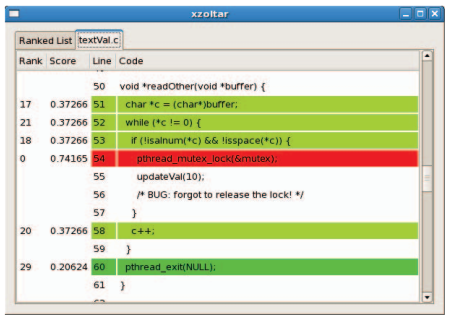
\includegraphics[width=6cm]{zoltar.png}
		\caption{\label{fig:zoltar} Example of Zoltar Interface \cite{janssen2009zoltar}}
	\end{center}
\end{figure}

In contrast to Zoltar, which was used to analyze programs written in C and C++,
CharmFL, is a Python tool that performs SBFL to identify faults. Sarhan et al.
\cite{sarhan2021charmfl} introduce CharmFL in a study that
discusses its features and implementation. The study recognizes the need for
SBFL tools to assist Python developers since it has become a very popular
language. Additionally, it presents CharmFL as a plugin for the popular IDE and
text editor PyCharm. Similar to AFLuent, it uses the Pytest framework to collect
program spectra and calculates suspiciousness scores using Tarantula, Ochiai,
and DStar approaches. Overall, CharmFL has many similarities with AFLuent, but
it's also less accessible considering that it's a PyCharm plugin which is not
used by every developer. Overall, the implementation of CharmFL provides and
inspiration for AFLuent and encourages improvements where CharmFL may fall
short.

\begin{figure}[!htb]
	\begin{center}
		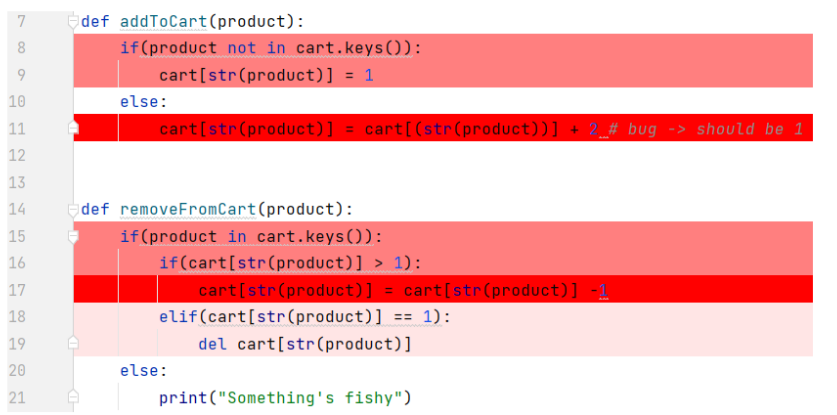
\includegraphics[width=10cm]{CharmFL.png}
		\caption{\label{fig:charmfl} Example interface of CharmFL \cite{sarhan2021charmfl}}
	\end{center}
\end{figure}

% TODO: requires more expansion
\section{Usability and Accessibility}
\label{sec:usability_accessibility}

Considering that the focus of AFLuent is not to simply be a fault localization
tool but rather an accessible one for beginner and novice developers, it's
important to better understand how the tool can be catered to that audience.
This can be done in many different ways, one of which is to increase the clarity
and verbosity of output messages from the tool. Instead of simply displaying the
ranked scores of statements, it would be more user friendly to explain the
meaning of the output to guide the user into beginning the debugging process.
Kohn \cite{kohn2019error} explores the experience of beginner with Python errors
with different severity and various Python interpreter error output. The results
confirm that more clear error messages tend to have a higher percentage of
students finding and fixing the error. This connection between error output and
the ability for beginner developers to fix faults is very crucial in the case of
AFLuent. And while a user survey is out of scope of this research, it's Kohn
provides encouragement to account for the different use cases in AFLuent and
attempt to provide a clear output that describes the fault and guides the
developer for the next step.

Another aspiration of AFLuent is to assist beginners in debugging their code in
ways that go beyond simply looking at the suspiciousness ranking of elements. By
identifying popular python errors in Python among beginners, cause of faults can
more quickly be pointed out after statement ranking has been produced. These
steps require additional analysis of the suspicious statements by analyzing
their syntax to identify potential cause. The goal of AFLuent would then become
more than simply locating the fault, but also giving an educated guess regarding
the reason behind the error. Cosman et al. \cite{cosman2020pablo} create a tool
named PABLO that uses a trained classifier to identify common bugs and faults in
beginner written Python programs. PABLO is also evaluated using an empirical and
human study to analyze how accurate it is in detecting mistakes and how helpful
users find the tool. Overall, PABLO is found to be ``helpful, providing
high-accuracy fault localization that implicates the correct terms
59-77\% of the time''. The ability of PABLO to describe the cause of error is
very valuable to incorporate in AFLuent, especially that AFLuent is only able to
conclude that there is an error and where it's possibly located. PABLO provides
another layer of fault localization that can only enhance the user experience.


%\numberedchapter{Method Of Approach}
\chapter{Method of Approach}
\label{ch:method}

This chapter describes the implementation of AFLuent and the experiment setup and
execution process. More specifically, the reasoning behind design decisions and
the result are the main focus. Additionally, charts and diagrams  are used to
demonstrate the the algorithms, structure, and flow of execution.

\section{Development Environment and Toolset}
\label{sec:DevEnviron}

Prior to explain how implementation was completed, a ground-up overview of the
tools used and their roles is necessary to establish definitions and facilitate
the understanding of how dependencies they are connected. AFLuent being a Python
tool allows its development to rely on a wide variety of helpful and popular
tools. Some of the most important tools and dependencies are discussed below.

\subsection{Poetry}
\label{subsec:poetry}

Poetry is a Python virtual environment management tool that allows developers to
set up an isolated environment for their projects. Furthermore, it manges the
installation of Python dependencies on the virtualenv and updates them when
necessary. Poetry has a crucial role in the implementation of AFLuent since it's
used to make the development process simpler, its role also goes beyond
that to the packaging and publishing of AFLuent to the Python Package Index
(PyPI). Poetry's ability to abstract and simplify all the details in creating a
Python package, makes it essential for development. However, from a user's
perspective, Poetry is not necessary to run or use the tool for fault localization.

\subsection{Pytest}
\label{subsec:pytest}

Pytest is a Python testing framework used to write and execute a variety of
tests, especially unit tests. Many developers in the community have contributed
to Pytest through plugins that extend Pytest's functionality and allow it to
accomplish new beneficial tasks. As mentioned previously, AFLuent is a Pytest
plugin that adds automated fault localization features. By definition, AFLuent
relies on Pytest in order to function properly. More details on how AFLuet is
integrated with pytest can be found in Section \ref{sec:makingPytestPlugin}.

\subsection{Coverage.py}
\label{subsec:coverage}

Spectrum based fault localization requires data on code coverage and test
results in order to calculate and rank suspicious of elements in the code.
Coverage.py\cite{coverage_py_website} is a Python tool that provides an easy to use application
programming interface to collect that data. The tool also provides various
configuration for the user to skip certain file or directories from being
considered. AFLuent relies on this tool to calculate what's known as per-test
coverage. This data describes the lines of code covered by a single test case
and organized in an accessible way to find out the number of passing and failing
test cases that executed each line. Automated fault localization approaches
require this information in order to calculate suspiciousness scores and
Coverage.py can provide that relatively easily.

\subsection{Radon}
\label{subsec:radon}

Radon is a Python tool used to calculate metrics of code complexity.
Specifically, it's used in AFLuent to calculate cyclomatic complexity of some
elements to break ties in rankings. When the user requests that AFLuent
considers cyclomatic complexity to be considered when ranking lines, Radon is
used to create a dataset of complexity scores. Since single lines cannot have a
cyclomatic complexity score, they are assigned the score of the function they're
a part of. Furthermore, the dataset is organized to facilitate efficient
searching by the line number in question.

\subsection{Libcst}
\label{subsec:libcst}

In order to provide additional methods to breaking ties between element
rankings, Libcst is used to create and abstract syntax tree of the code in
question. This approach allows AFLuent to assess code complexity using the
code's syntax. Additional details on the use of Libcst are discussed in (planning
to add reference to a section.)
% TODO: add reference to the section discussing this

\section{AFLuent as a Pytest Plugin}
\label{sec:makingPytestPlugin}

\begin{figure}[!htb]
	\begin{center}
		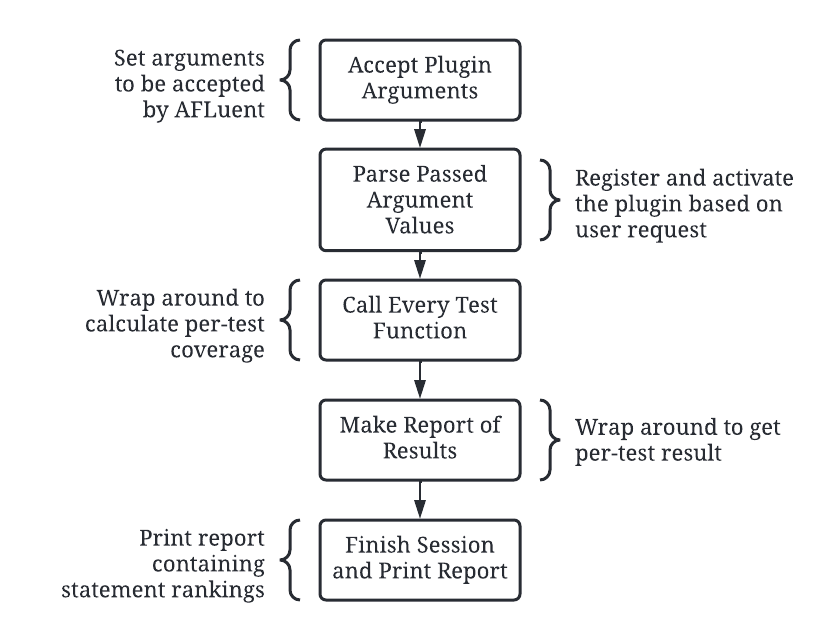
\includegraphics[width=11.9cm]{pytest_flowfchart.png}
		\caption{\label{fig:pytest_flow} Pytest Tasks Flowchart}
	\end{center}
\end{figure}

Pytest provides simple and intuitive ways of extending its functionality through
hooks. These hooks break up the standard Pytest execution steps and allow
external code to run at these points. A plugin is essentially a collection of
packaged hooks that fit in the workflow of Pytest. AFLuent makes use of five
different hooks to implement automated fault localization.
Fig.\ref{fig:pytest_flow} shows a general overview of the steps changed in the
workflow of Pytest. Additionally, the section below describes in details how each
step was modified.

\section{Installing AFLuent}
\label{subsec:afluent_install}

As part of the goal of creating a novice friendly tool, it's very important that
AFLuent can be installed and set up easily on any system with little to no
complications. To achieve that, AFLuent is published to the Python Package Index
(PyPI), which makes it installable through the \code{pip install afluent}
command. Once this command runs successfully, AFLuent is automatically
integrated with Pytest as a plugin and will be ran with every pytest session
unless otherwise disabled intentionally. AFLuent's dependency on Coverage.py
creates a small but avoidable conflict. In the case that AFluent and another plugin that
utilizes Coverage.py is active in the same Pytest session, various errors might
occur where coverage information is not calculated correctly, thus affecting the
automated fault localization process. This issue was prevalent when specifically
using \code{pytest-cov} plugin, which produces a coverage report at the end of a
Pytest session. AFLuent handles this problem by checking for the presence of
other Coverage.py reliant plugins and warns the user. Due to this issue,
AFLuent will not run in the session unless specified specifically using the
command-line arguments discussed in the following section.

\subsection{Adding Command-Line Arguments}
\label{subsec:pytest_cli}

Pytest already supports a multitude of command line arguments that allow the
user to pass configuration that change how the test suite is executed and
reported. Similarly, AFLuent requires user passed arguments to complete a
variety of tasks. The hook \code{pytest\_addoption} allows adding new
arguments in a fashion similar to the \code{argparse} Python library.
The \code{argparse} library supports features that allow easy parsing and validation of
command-line arguments. Furthermore, it facilitates working with input with
various data types.
The added arguments accept values that specify the following:
\begin{itemize}
    \item If AFLuent should be enabled for the current Pytest session.
    \begin{itemize}
        \item Flags: \code{---afl-debug} or \code{---afl}
    \end{itemize}
    \item The techniques for suspiciousness score calculations
%    TODO: add approaches to the list after implementation
    \begin{itemize}
        \item \code{---tarantula}: enable fault localization using Tarantula approach
        \item \code{---ochiai}: enable fault localization using Ochiai approach
        \item \code{---dstar}: enable fault localization using DStar approach
        \item \code{---dstar-pow}: used to set the power to use in the DStar
        approach. Defaults to 3
        \item Multiple approaches can be used at the same time, however, results
        will be sorted by the approach passed first.
    \end{itemize}
    \item The number of results to display in the report
    \begin{itemize}
        \item \code{---afl-results}: number of top results to show in the
        terminal window. Defaults to 20
    \end{itemize}
    \item The directories and files to be ignored while calculating coverage
    \begin{itemize}
        \item \code{---afl-ignore}: Used to pass directories and files to
        ignore. Example: \code{tests/*} will ignore all files and directories
        inside the \code{tests} folder.
    \end{itemize}
    \item The types of file reports to created after the Pytest session is over
    \begin{itemize}
        \item \code{---report}: accepts \code{json} or \code{csv} and generate
        reports with the passed format.
        \item \code{---per-test-report}: requires that a per-test coverage
        report is produced. This report is only generated in JSON format.
    \end{itemize}
    \item If complexity metrics should be used in breaking ties of ranked elements
    \begin{itemize}
        \item \code{---cyclomatic-complexity}: use cyclomatic complexity metrics
        in breaking ties found in suspiciousness scores
        \item \code{---syntax-complexity}: use syntax complexity metrics
        in breaking ties found in suspiciousness scores
    \end{itemize}
\end{itemize}

\subsection{Activating AFLuent}
\label{subsec:activate_afluent}

After arguments are passed, the next steps parses through some of them to check
if AFLuent was enabled and to validate some of their values. The Pytest hook
\code{pytest\_cmdline\_main} gives access to the collected configuration. In
this hook, checks are conducted to see if there are other active plugins that
utilize Coverage.py. These checks are necessary due to conflicts in collecting
data when multiple plugins use Coverage.py simultaneously. The problem is
resolved through warnings to the user that ask to disable these plugins in order
for AFLuent to run properly. Lastly, if AFLuent is enabled, an \code{Afluent} object is initialized
with the passed configuration and registered as a plugin for the current Pytest session.

\subsection{Calculating Per-test Coverage and Test Result}
\label{subsec:calculate_coverage}

Per-test coverage is defined here as the collection of lines executed by
each individual test case. In order to collect this data, AFLuent adds a wrapper
that executes code before and after each test case function is called. The
\code{pytest\_pyfunc\_call} hook is used in this scenario. The execution steps
are as follows:

\begin{enumerate}
    \item \code{cov.start()} begins recording coverage
    \item the hook yields back control to Pytest which calls the individual test case
    \item \code{cov.stop()} stops recording coverage
    \item The collected data is then organized in a simpler structure defined as
    the program spectra
    \item The process repeats for every test case
\end{enumerate}

Once per-test coverage is completed, the \code{pytest\_runtest\_makereport} hook
is used to get the outcome of each test case and add it to the program spectra
structure. There are three possible test outcome in Pytest, `Passed', `Failed',
and `Skipped'.

\subsection{Reporting Results}
\label{subsec:report_results}

The last step in AFLuent execution as part of Pytest is to report the fault
localization outcome. The \code{pytest\_sessionfinish} hook is used to detect the
exit code of the session and display output on the console accordingly. An exist
code of 0 means that all tests have passed and there is no need to perform fault
localization, therefore, a message would display that to the user before
finishing the Pytest run. On the other hand an exit code of 1, would indicate
that at least one test case failed during the pytest session. In this scenario,
AFLuent initializes a \code{Spectrum} object, which is responsible for parsing
through the program spectra structure, ranking elements based on suspiciousness,
and producing an output to the console.

\section{AFLuent's Components}
\label{sec:components}

Considering all the steps involved in calculating and reporting suspiciousness
of elements, AFLuent is implemented in an object oriented style that focuses on
the readability and maintainability of the code. By splitting up AFLuent to a
collection of objects organized in a hierarchy, the testing approach becomes more
clear and debugging becomes easier. This section discusses the objects oriented
structure starting with the least complex.

\subsection{Line Object}
\label{subsec:line_obj}

A line is the simplest unit in a large project or program. With that in mind, a
\code{Line} object describes the attributes and implements the functionalities
associated with a single line in the context of automated fault localization.
Important attributes of a line include identifiers such as the line number and
file path it belongs to. Other line-specific information include a list of
failed test cases that executed this line, and another for tests that passed.
This information is crucial in calculating the one of the main focuses of
AFLuent, which is suspiciousness scores. These scores are also stored as
attributes of each Line object. Another stored attribute is complexity,
which is a metric associated with each line and used to break ties in rankings.
Further reading on complexity metrics can be found in REFERENCE TO BE DETERMINED
% TODO: requires elaboration

As for functions, a Line object contains an implementation of the three
equations, Tarantula shown in Fig.\ref{fig:tarantulaEquation}, Ochiai shown in
Fig.\ref{fig:ochiaiEquation}, and DStar shown in Fig.\ref{fig:dstarEquation},
where suspiciousness scores are calculated and rounded up to four decimal places.
The mathematical implementations of these functions also handle and account for
division by zero. Depending on the equation, there could be multiple instances
where division by zero is possible. The following subsections discuss how this
issue was handled for each equation.

% TODO: the number of equations should be updated once new ones are added

\subsubsection{Division by Zero: Tarantula}
\label{subsubsec:div_by_zero_taran}
In the Tarantula equation, division by zero occurs if either the number of
total passing tests or number of total failing tests is zero. In the case that
there are no failing test-cases in the whole test suite, then the suspiciousness
of all covered statements is zero (not suspicious) since there was no fault. The
other edge case occurs when there are no passing tests in the whole test suite,
in which every covered line has the maximum suspiciousness of 1. It is important
to acknowledge that the outcomes reached here only apply to code that has been
covered by the test suite. Faulty lines, which are not covered by any test case
will not be investigated since there is no data to calculate their
suspiciousness. Using values plugged in to Fig.\ref{fig:tarantulaEquation}, the
examples in Fig.\ref{fig:taran_div_by_zero_1} and Fig.\ref{fig:taran_div_by_zero_2} show
the two possible cases where division by zero might occur in the Tarantula
equation.

\begin{figure}[!htb]
	\begin{center}
        When \textbf{N$_{CF}$ = 0} and \textbf{N$_{UF}$ = 0 }
		\begin{equation}
			Tarantula(element) = \frac{\frac{\textbf{0}}{\textbf{0}}}{\frac{\textbf{N$_{CS}$}}{\textbf{N$_{CS}$}+\textbf{N$_{US}$}} + \frac{\textbf{0}}{\textbf{0}}}
		\end{equation}
		\caption{\label{fig:taran_div_by_zero_1} Tarantula Division by Zero Example 1}
	\end{center}
\end{figure}

\begin{figure}[!htb]
	\begin{center}
        When \textbf{N$_{CS}$ = 0} and \textbf{N$_{US}$ = 0 }
		\begin{equation}
			Tarantula(element) = \frac{\frac{\textbf{N$_{CF}$}}{\textbf{N$_{CF}$} + \textbf{N$_{UF}$}}}{\frac{\textbf{0}}{\textbf{0}} + \frac{\textbf{N$_{CF}$}}{\textbf{N$_{CF}$}+\textbf{N$_{UF}$}}}
		\end{equation}
		\caption{\label{fig:taran_div_by_zero_2} Tarantula Division by Zero Example 2}
	\end{center}
\end{figure}

Fig.\ref{fig:taran_div_by_zero_1} shows the case where there is a total of zero
failed test cases, covering AND not covering the element, in which a score
of 0 is assigned to the element. On the other hand,
Fig.\ref{fig:taran_div_by_zero_2} shows the case where there is a total of zero
passing test cases, in which a maximum score of 1 is assigned to the element.

\subsubsection{Division by Zero: Ochiai}
\label{subsubsec:div_by_zero_ochiai}

Division by zero occurs in the Ochiai formula when there is not test coverage
information for a line or when the total number of failed tests is zero.
The latter case indicates that the line is not suspicious since it did not
cause any failures, therefore, zero is returned as the suspiciousness score.
However, the former case is not considered at all since AFLuent does not include
lines with no coverage information.
Fig.\ref{fig:ochiai_div_by_zero_1} and Fig.\ref{fig:ochiai_div_by_zero_2}
demonstrates that equation after plugging in
the zero values from \ref{fig:ochiaiEquation}

\begin{figure}[!htb]
	\begin{center}
        When \textbf{N$_{CF}$ = 0} and \textbf{N$_{UF}$ = 0 }
		\begin{equation}
			Ochiai(element) = \frac{\textbf{0}}{\sqrt{(\textbf{0}) \cdot (\textbf{0}  + \textbf{N$_{CS}$})}}
		\end{equation}
		\caption{\label{fig:ochiai_div_by_zero_1} Ochiai Division by Zero Example 1}
	\end{center}
\end{figure}

\begin{figure}[!htb]
	\begin{center}
        When \textbf{N$_{CF}$ = 0} and \textbf{N$_{CS}$ = 0 }
		\begin{equation}
			Ochiai(element) = \frac{\textbf{0}}{\sqrt{(\textbf{0}  + \textbf{N$_{UF}$}) \cdot (\textbf{0})}}
		\end{equation}
		\caption{\label{fig:ochiai_div_by_zero_2} Ochiai Division by Zero Example 2}
	\end{center}
\end{figure}

Fig.\ref{fig:ochiai_div_by_zero_1} is an example of when there is zero total
failed test cases, resulting in a zero suspiciousness score.
However Fig\ref{fig:ochiai_div_by_zero_2} shows an example where there is no
failed or successful tests that cover the line. This scenario does not
occur in AFLuent, which only looks at lines that have some coverage data through
passing or failing tests. Therefore, it wasn't necessary to handle this possibility.

\subsubsection{Division by Zero: DStar}
\label{subsubsec:div_by_zero_dstar}

In the DStar equation, division by zero takes place only in one case. When the
number of passing test cases that cover the line AND the number of failed test
cases that do not cover the line are both zero, the denominator evaluates to
zero. This translates to the following: if there is no passing tests executing
this line and no failing test executing other lines only, then this line should
have the maximum suspiciousness score possible. However, since DStar has a
numerator raised to a power set by the user, it has no numerical upper limit on
the resulting score. To resolve this issue, the maximum integer value is
assigned as the suspiciousness score of this line.
Fig.\ref{fig:dstar_div_by_zero} shows and example of this scenario after
plugging in values from Fig.\ref{fig:dstarEquation}

\begin{figure}[!htb]
	\begin{center}
        When \textbf{N$_{CS}$ = 0} and \textbf{N$_{UF}$ = 0 }
		\begin{equation}
			Dstar(element) = \frac{(\textbf{N$_{CF}$})^{\ast}}{\textbf{0}}
		\end{equation}
		\caption{\label{fig:dstar_div_by_zero} DStar Division by Zero Example}
	\end{center}
\end{figure}

\subsection{ProjFile Object}
\label{subsec:projfile_obj}

ProjFile objects are designed to contain attributes that describe whole files.
Additionally, they support functionality that apply to these files. The most
important attributes of these objects is the \code{lines} instance variable,
which stores a dictionary of contents of the file. Specifically, the keys in
this dictionary are line numbers in the file and the values are the Line objects
discussed previously. In addition to storing this data, ProjFile implements an
intuitive way to update it with a new result of a test case. \code{update\_file}
function takes in a list of numbers of covered lines executed by a test case as well as the
result and the name of that test case. Following that, it iterates through the
covered line numbers and updates the Line objects stored in the ProjFile
dictionary. This approach creates a hierarchy between the objects by nesting
Line objects inside of ProjFile objects.

\subsection{Spectrum Object}
\label{subsec:spectrum_obj}

This object contains some of the core functionalities that organizes the
collected data and displays it to the console. Similar to how a ProjFile object
stores a dictionary of line number and Line object pairs, Spectrum takes nesting
a step further and stores a dictionary of file paths and ProjFile objects as
key-value pairs. Additionally, it keeps track of running totals of passed,
failed, and skipped test cases, which are used to calculate suspiciousness
scores. Lastly, it's responsible for sorting Line objects in a descending order
from highest suspiciousness scores. Once this task is completed, the Spectrum
object produces a table formatted report with color coded results that
demonstrate to the user the outcome of fault localization.
% TODO: discuss more about the report structure and colors and give figure example

\subsection{Afluent Object}
\label{subsec:afluent_obj}

While this Object does not implement any functionality regarding the calculation
or sorting of suspiciousness scores, it plays an important role in integrating
this tool with Pytest. By containing several of the Pytest hooks mentioned
prior, this object is registered as the plugin when AFLuent is enabled through
command line arguments. Following the end of the Pytest session, the AFluent
object initializes a Spectrum Object and forwards the arguments collected from
the console command. Following that, it calls the Spectrum object to produce and
print its report. Overall, this object acts as a pipeline that passes coverage
information and command line arguments collected from the Pytest session to the
infrastructure responsible for performing fault localization.

\subsection{Objects Overview}
\label{subsec:obj_overview}

\begin{figure}[!htb]
	\begin{center}
		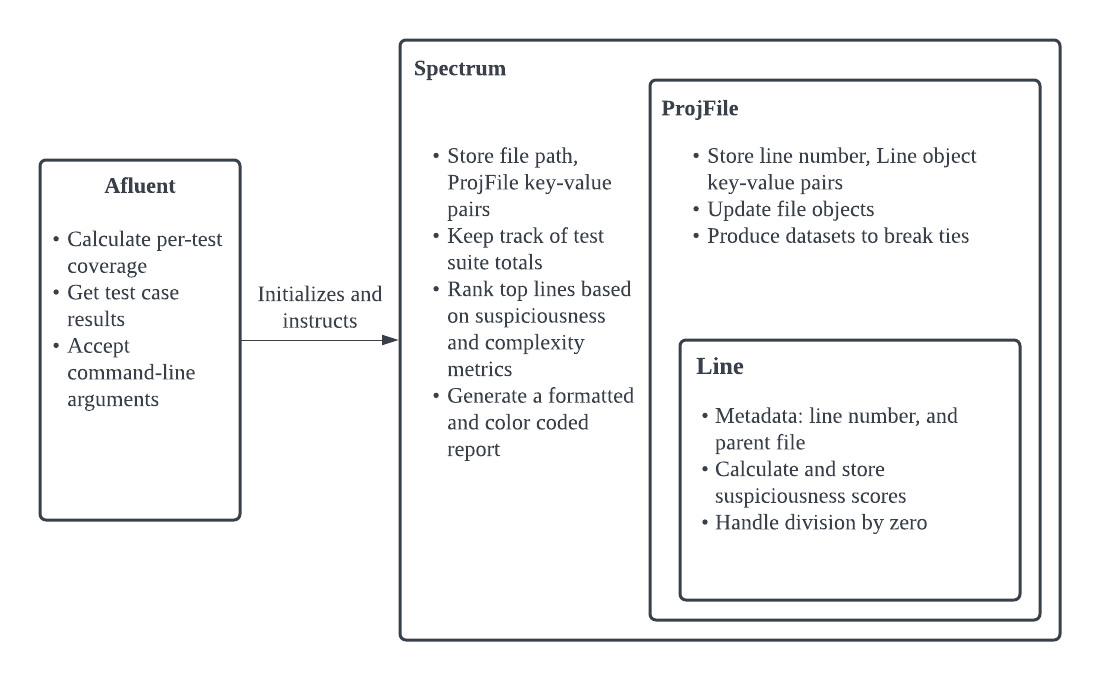
\includegraphics[width=15.5cm]{object_oriented_structure.png}
		\caption{\label{fig:oop_structure} AFLuent Object Structure}
	\end{center}
\end{figure}

Fig\ref{fig:oop_structure} provides a visual simplification of the different
components of AFluent and an overview of their roles in the functioning of the
tool. Overall the nested structure creates several layers that facilitate
development by isolating the different components and hiding unnecessary
information from other objects in the hierarchy.

%\numberedchapter{Experimental Results}
\chapter{Experimental Results} 
\label{ch:experiments}

This chapter should describe your experimental set up and evaluation. It should also produce and describe the results of your study. Possible section titles are given below.

\section{Experimental Design}

\section{Evaluation}

\section{Threats to Validity}

%\numberedchapter{Conclusion}
\chapter{Discussion and Future Work}  
\label{ch:conclusion}

This is the conclusion. You might want to leave it unnumbered, as it is now. If you want to number it, treat it like any other chapter.

This chapter usually contains the following items, although not
necessarily in this order or sectioned this way in particular.

\section{Summary of Results}
A discussion of the significance of the results
and a review of claims and contributions.

\section{Future Work}
\label{sec:future_work}

\section{Conclusion}


 
%----------------------------------------------------------------------------------------
%	BIBLIOGRAPHY
%----------------------------------------------------------------------------------------

\addtocontents{toc}{\vspace{2em}} % Add a gap in the Contents, for aesthetics
\unnumberedchapter{Bibliography} % Title of the unnumbered chapter
\bibliography{preamble/bibliography} % The references information are stored in the file named "bibliography.bib"


\end{document}  